\section{Future work}
\label{sec:future}

\subsection{Direct addressing for partially-structured meshes}
\label{sec:future_partialstructure}

% stand to make a small memory saving - affects prefetch, loop unrolling, working set size, bandwidth stuff
% not necessarily worth it... but permitted by abstraction

% below are unified by "mesh transformation" approach in DMPlex - should be possible to reconstruct
% data hierarchy by inspecting labels.

\subsubsection{Extruded meshes}

\subsubsection{Regular mesh refinement}

% refinement 1
\begin{tikzpicture}

  \tkzDefPoint(0,0){v0}
  \tkzDefShiftPoint[v0](60:4){v1}
  \tkzDefShiftPoint[v0](0:4){v2}
  \tkzDrawPolygon(v0,v1,v2)

  \tkzLabelPoint[below left](v0){$v_0$}
  \tkzLabelPoint[above](v1){$v_1$}
  \tkzLabelPoint[below right](v2){$v_2$}

  \tkzLabelSegment(v0,v1){$e_0$}
  \tkzLabelSegment(v1,v2){$e_1$}
  \tkzLabelSegment(v2,v0){$e_2$}

  \tkzDefBarycentricPoint(v0=1,v1=1,v2=1) \tkzGetPoint{c0}
  \tkzLabelPoint[centered](c0){$c_0$}

\end{tikzpicture}

\vspace{1em}

% refinement 2
\begin{tikzpicture}

  \tkzDefPoint(0,0){v0}
  \tkzDefShiftPoint[v0](60:4){v1}
  \tkzDefShiftPoint[v0](0:4){v2}
  \tkzDrawPolygon(v0,v1,v2)

  \tkzDefMidPoint(v0,v1) \tkzGetPoint{e0v0}
  \tkzDefMidPoint(v1,v2) \tkzGetPoint{e1v0}
  \tkzDefMidPoint(v2,v0) \tkzGetPoint{e2v0}

  \tkzDrawSegment(e0v0,e1v0)
  \tkzDrawSegment(e1v0,e2v0)
  \tkzDrawSegment(e2v0,e0v0)

  % note: this method is outdated - bisect instead
  \begin{pgfonlayer}{background}
    \tkzDefBarycentricPoint(e0v0=25,v1=1,e1v0=1,e2v0=1) \tkzGetPoint{e0v0inner}
    \tkzDefBarycentricPoint(e0v0=1,v1=25,e1v0=1,e2v0=1) \tkzGetPoint{v1inner}
    \tkzDefBarycentricPoint(e0v0=1,v1=1,e1v0=25,e2v0=1) \tkzGetPoint{e1v0inner}
    \tkzDefBarycentricPoint(e0v0=1,v1=1,e1v0=1,e2v0=25) \tkzGetPoint{e2v0inner}


    \draw[rounded corners] (e0v0inner) -- (v1inner) -- (e1v0inner) -- (e2v0inner) -- cycle;
  \end{pgfonlayer}

\end{tikzpicture}

% \vspace{1em}
\pagebreak

% refinement 3
\begin{tikzpicture}

  \tkzDefPoint(0,0){v0}
  \tkzDefShiftPoint[v0](60:4){v1}
  \tkzDefShiftPoint[v0](0:4){v2}
  \tkzDrawPolygon(v0,v1,v2)

  \tkzDefMidPoint(v0,v1) \tkzGetPoint{e0v0}
  \tkzDefMidPoint(v1,v2) \tkzGetPoint{e1v0}
  \tkzDefMidPoint(v2,v0) \tkzGetPoint{e2v0}

  \tkzDrawSegment(e0v0,e1v0)
  \tkzDrawSegment(e1v0,e2v0)
  \tkzDrawSegment(e2v0,e0v0)

  \tkzDefMidPoint(e1v0,v2) \tkzGetPoint{e1e1v0}
  \tkzDefMidPoint(v2,e2v0) \tkzGetPoint{e2e0v0}
  \tkzDefMidPoint(e1v0,e2v0) \tkzGetPoint{c0e2v0}

  \tkzDrawSegment(e1e1v0,e2e0v0)
  \tkzDrawSegment(e2e0v0,c0e2v0)
  \tkzDrawSegment(c0e2v0,e1e1v0)

  % patch
  \begin{pgfonlayer}{background}
    % find points by bisecting the angles
    \tkzDefShiftPoint[e0v0](-30:0.15){e0v0inner}
    \tkzDefShiftPoint[e1v0](-120:0.1){e1v0inner}
    \tkzDefShiftPoint[e1e1v0](150:0.15){e1e1v0inner}
    \tkzDefShiftPoint[c0e2v0](120:0.1){c0e2v0inner}
    \tkzDefShiftPoint[e2v0](90:0.15){e2v0inner}

    % source: https://tikz.dev/base-paths#sec-102.12
    \pgfsetcornersarced{\pgfpoint{1mm}{1mm}}
    \filldraw[color=blue!20] (e0v0inner) -- (e1v0inner) -- (e1e1v0inner) -- (c0e2v0inner) -- (e2v0inner) -- cycle;
    \pgfsetcornersarced{\pgfpointorigin}
  \end{pgfonlayer}

  % add labels
  \tkzDefBarycentricPoint(e0v0=1,e1v0=1,e2v0=1) \tkzGetPoint{c0c1}
  \node [xshift=-2cm,yshift=.8cm] (c0c1label) at (c0c1) {$(c_i,c_1)$};
  \draw (c0c1label) -- (c0c1);

  \tkzDefMidPoint(e1v0,c0e2v0) \tkzGetPoint{c0e2}
  \node [xshift=2cm,yshift=.8cm] (c0e2label) at (c0e2) {$(c_i,e_2,e_0)$};
  \draw (c0e2label) -- (c0e2);

  \tkzDefBarycentricPoint(e1v0=1,e1e1v0=1,c0e2v0=1) \tkzGetPoint{c0c3c2}
  \node [xshift=2cm,yshift=-.2cm] (c0c3c2label) at (c0c3c2) {$(c_i,c_3,c_2)$};
  \draw (c0c3c2label) -- (c0c3c2);

\end{tikzpicture}

\vspace{2em}

% data layout for patch
\begin{tikzpicture}[y=-1cm]
  \begin{scope}[xshift=1.5cm, yshift=0cm]
    \fill[lightgray] (0,0) rectangle (4,1);
    \filldraw[draw=black, fill=white] (1.5,0) rectangle ++ (1,1);
    \node[at={(2,.5)}, ptlabel] {$c_i$};
    \draw (0,0) -- (4,0);
    \draw (0,1) -- (4,1);
  \end{scope}

  \begin{scope}[xshift=.5cm, yshift=-2cm]
    \filldraw[draw=black, fill=white] (0,0) rectangle ++ (1,1);
    \filldraw[draw=black, fill=blue!20] (1,0) rectangle ++ (1,1);
    \filldraw[draw=black, fill=white] (2,0) rectangle ++ (1,1);
    \filldraw[draw=black, fill=white] (3,0) rectangle ++ (1,1);
    \filldraw[draw=black, fill=white] (4,0) rectangle ++ (1,1);
    \filldraw[draw=black, fill=white] (5,0) rectangle ++ (1,1);
    \filldraw[draw=black, fill=white] (6,0) rectangle ++ (1,1);
    \node[at={(.5,.5)}, ptlabel] {$c_0$};
    \node[at={(1.5,.5)}, ptlabel] {$c_1$};
    \node[at={(2.5,.5)}, ptlabel] {$c_2$};
    \node[at={(3.5,.5)}, ptlabel] {$c_3$};
    \node[at={(4.5,.5)}, ptlabel] {$e_0$};
    \node[at={(5.5,.5)}, ptlabel] {$e_1$};
    \node[at={(6.5,.5)}, ptlabel] {$e_2$};

    % \draw[->] (2.8,-1) .. controls ([yshift=-.4cm] 2.6,-1) and ([yshift=.6cm] 1,0) .. (.8,0);
    % \draw[->] (3,-1) .. controls ([yshift=-.6cm] 3,-1) and ([yshift=1cm] 3.5,0) .. (3.5,0);
    % \draw[->] (3.2,-1) .. controls ([yshift=-.4cm] 3,-1) and ([yshift=.6cm] 6,0) .. (6.2,0);
  \end{scope}

  \begin{scope}[xshift=0cm, yshift=-4cm]
    % c3
    \begin{scope}[xshift=0cm]
      \fill[lightgray] (0,0) rectangle (4,1);
      \filldraw[draw=black, fill=white] (.5,0) rectangle ++ (1,1);
      \filldraw[draw=black, fill=blue!20] (1.5,0) rectangle ++ (1,1);
      \filldraw[draw=black, fill=white] (2.5,0) rectangle ++ (1,1);
      \node[at={(1,.5)}, ptlabel] {$c_1$};
      \node[at={(2,.5)}, ptlabel] {$c_2$};
      \node[at={(3,.5)}, ptlabel] {$c_3$};
      \draw (0,0) -- (4,0);
      \draw (0,1) -- (4,1);
      % \draw[->] (4,-1) .. controls ([yshift=-.7cm] 4,-1) and ([yshift=1cm] 2,0) .. (2,0);
    \end{scope}

    % e2
    \begin{scope}[xshift=5cm]
      \filldraw[draw=black, fill=blue!20] (0,0) rectangle ++ (1,1);
      \filldraw[draw=black, fill=white] (1,0) rectangle ++ (1,1);
      \filldraw[draw=black, fill=white] (2,0) rectangle ++ (1,1);
      \node[at={(.5,.5)}, ptlabel] {$e_0$};
      \node[at={(1.5,.5)}, ptlabel] {$e_1$};
      \node[at={(2.5,.5)}, ptlabel] {$v_0$};
      % \draw[->] (2,-1) .. controls ([yshift=-.7cm] 2,-1) and ([yshift=1cm] .5,0) .. (.5,0);
    \end{scope}
  \end{scope}

  \draw ({1.5+1.5},1) -- ({0+.5},2);
  \draw ({2.5+1.5},1) -- ({7+.5},2);

  \draw ({2+1.5},3) -- ({0+0},4);
  \draw ({3+1.5},3) -- ({4+0},4);

  \draw ({5+1.5},3) -- ({0+5},4);
  \draw ({6+1.5},3) -- ({3+5},4);
\end{tikzpicture}

\vspace{2em}


\vspace{2em}

% alt refinement 3
\begin{tikzpicture}

  \tkzDefPoint(0,0){v0}
  \tkzDefShiftPoint[v0](60:4){v1}
  \tkzDefShiftPoint[v0](0:4){v2}
  \tkzDrawPolygon(v0,v1,v2)

  \tkzDefMidPoint(v0,v1) \tkzGetPoint{e0v0}
  \tkzDefMidPoint(v1,v2) \tkzGetPoint{e1v0}
  \tkzDefMidPoint(v2,v0) \tkzGetPoint{e2v0}

  \tkzDrawSegment(e0v0,e1v0)
  \tkzDrawSegment(e1v0,e2v0)
  \tkzDrawSegment(e2v0,e0v0)

  \tkzDefMidPoint(e1v0,v2) \tkzGetPoint{e1e1v0}
  \tkzDefMidPoint(v2,e2v0) \tkzGetPoint{e2e0v0}
  \tkzDefMidPoint(e1v0,e2v0) \tkzGetPoint{c0e2v0}

  \tkzDrawSegment(e1e1v0,e2e0v0)
  \tkzDrawSegment(e2e0v0,c0e2v0)
  \tkzDrawSegment(c0e2v0,e1e1v0)

  \tkzDrawSegment(e0v0,c0e2v0)
\end{tikzpicture}

\vspace{1em}
% vertex refinement
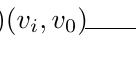
\begin{tikzpicture}

  \tkzDefPoint(0,0){cvert}
  \tkzDrawPoint(cvert) \tkzLabelPoint[above](cvert){$(v_i,)$}

  \draw[->] (1,0) -> (2,0);

  \tkzDefPoint(3,0){fvert}
  \tkzDrawPoint(fvert) \tkzLabelPoint[above](fvert){$(v_i,v_0)$}


\end{tikzpicture}

\vspace{2em}

% edge refinement
\begin{tikzpicture}

  \tkzDefPoint(0,0){cstart}
  \tkzDefPoint(3,0){cend}
  \tkzDrawSegment(cstart,cend)
  \tkzLabelSegment(cstart,cend){$(e_i,)$}

  \draw[->] (4,0) -> (5,0);

  \tkzDefPoint(6,0){fstart}
  \tkzDefPoint(11,0){fend}
  \tkzDefMidPoint(fstart,fend) \tkzGetPoint{fmid}

  \tkzDrawSegment(fstart,fmid) \tkzLabelSegment(fstart,fmid){$(e_i,e_0)$}
  \tkzDrawSegment(fmid,fend) \tkzLabelSegment(fmid,fend){$(e_i,e_1)$}
  \tkzDrawPoint(fmid) \tkzLabelPoint[below](fmid){$(e_i,v_0)$}

\end{tikzpicture}

\vspace{2em}

% cell refinement
\begin{tikzpicture}

  \tkzDefPoint(0,0){v0}
  \tkzDefShiftPoint[v0](60:5){v1}
  \tkzDefShiftPoint[v0](0:5){v2}
  \tkzDrawPolygon[style=dashed](v0,v1,v2)

  \tkzDefBarycentricPoint(v0=1,v1=1,v2=1) \tkzGetPoint{c0}
  \tkzLabelPoint[centered](c0){$c_i$}

  \draw[->] (5,{5/4*sqrt(3)}) -- (6,{5/4*sqrt(3)});

  \tkzDefPoint(7,0){fv0}
  \tkzDefShiftPoint[fv0](60:5){fv1}
  \tkzDefShiftPoint[fv0](0:5){fv2}
  \tkzDrawPolygon[style=dashed](fv0,fv1,fv2)

  \tkzDefMidPoint(fv0,fv1) \tkzGetPoint{fe0}
  \tkzDefMidPoint(fv1,fv2) \tkzGetPoint{fe1}
  \tkzDefMidPoint(fv2,fv0) \tkzGetPoint{fe2}

  \tkzDrawSegment(fe0,fe1)
  \tkzDrawSegment(fe1,fe2)
  \tkzDrawSegment(fe2,fe0)

  \tkzDefBarycentricPoint(fv0=1,fe0=1,fe2=1) \tkzGetPoint{fc0}
  \tkzLabelPoint[centered](fc0){$(c_i,c_0)$}

  \tkzDefBarycentricPoint(fe0=1,fe1=1,fe2=1) \tkzGetPoint{fc1}
  \tkzLabelPoint[centered](fc1){$(c_i,c_1)$}

  \tkzDefBarycentricPoint(fv1=1,fe0=1,fe1=1) \tkzGetPoint{fc2}
  \tkzLabelPoint[centered](fc2){$(c_i,c_2)$}

  \tkzDefBarycentricPoint(fv2=1,fe1=1,fe2=1) \tkzGetPoint{fc3}
  \tkzLabelPoint[centered](fc3){$(c_i,c_3)$}

  % edges (2/3 along)
  \tkzDefBarycentricPoint(fe2=1,fe0=2) \tkzGetPoint{e0labeldest}
  \tkzDefBarycentricPoint(fe0=1,fe1=2) \tkzGetPoint{e1labeldest}
  \tkzDefBarycentricPoint(fe1=2,fe2=1) \tkzGetPoint{e2labeldest}

  \node [xshift=-1.6cm,yshift=.2cm] (e0labelsrc) at (e0labeldest) {$(c_i,e_0)$};
  \draw (e0labelsrc) -- (e0labeldest);

  \node [xshift=1.2cm,yshift=.9cm] (e1labelsrc) at (e1labeldest) {$(c_i,e_1)$};
  \draw (e1labelsrc) -- (e1labeldest);

  \node [xshift=1.5cm,yshift=.4cm] (e2labelsrc) at (e2labeldest) {$(c_i,e_2)$};
  \draw (e2labelsrc) -- (e2labeldest);



\end{tikzpicture}

\subsection{Data layout transformations}

% mixed reordering
\begin{tikzpicture}[y=-1cm]
  \begin{scope}[xshift=3.5cm, yshift=0cm]
    \filldraw[draw=black, fill=white] (0,0) rectangle (1,1);
    \filldraw[draw=black, fill=white] (1,0) rectangle (2,1);
    \node[at={(.5,.5)}, ptlabel] {$V_0$};
    \node[at={(1.5,.5)}, ptlabel] {$V_1$};
  \end{scope}

  \begin{scope}[yshift=-2cm]
    \begin{scope}[xshift=0cm]
      \fill[lightgray] (0,0) rectangle (4,1);
      \filldraw[draw=black, fill=white] (0.5,0) rectangle (1.5,1);
      \filldraw[draw=black, fill=white] (1.5,0) rectangle (2.5,1);
      \filldraw[draw=black, fill=white] (2.5,0) rectangle (3.5,1);
      \node[at={(1,.5)}, ptlabel] {$c_0$};
      \node[at={(2,.5)}, ptlabel] {$v_1$};
      \node[at={(3,.5)}, ptlabel] {$c_4$};
      \draw (0,0) -- (4,0);
      \draw (0,1) -- (4,1);
    \end{scope}

    \begin{scope}[xshift=5cm]
      \fill[lightgray] (0,0) rectangle (4,1);
      \filldraw[draw=black, fill=white] (0.5,0) rectangle (1.5,1);
      \filldraw[draw=black, fill=white] (1.5,0) rectangle (2.5,1);
      \filldraw[draw=black, fill=white] (2.5,0) rectangle (3.5,1);
      \node[at={(1,.5)}, ptlabel] {$c_0$};
      \node[at={(2,.5)}, ptlabel] {$v_1$};
      \node[at={(3,.5)}, ptlabel] {$c_4$};
      \draw (0,0) -- (4,0);
      \draw (0,1) -- (4,1);
    \end{scope}
  \end{scope}

  \draw (3.5,1) -- (0,2);
  \draw (4.5,1) -- (4,2);
  \draw (4.5,1) -- ({0+5},2);
  \draw (5.5,1) -- ({4+5},2);

\end{tikzpicture}

% one could introduce a proper tensor language to express things (like Simit) - currently only
% focussed on the packing part
\subsection{Orienting degrees-of-freedom}

One significant challenge stencil applications face when applied to \glspl{pde} is on agreeing on a consistent orientation of the \glspl{dof} for shared entities.
% introduce ``reference'' as a term
%Note that we use the term ``reference'' here to mean ``the canonical arrangement of \glspl{dof} that is expected by the local kernel''.

To demonstrate the issue, consider the \gls{dof} arrangements shown in Figure~\ref{fig:orient}.
Figures~\ref{fig:orient_basic_ref} and~\ref{fig:orient_vector_ref} show the reference \gls{dof} arrangements for an arbitrary space on triangles, with scalar or vector \glspl{dof} on the edges respectively.
Likewise, Figures~\ref{fig:orient_basic_flip} and~\ref{fig:orient_vector_flip} show the resulting \gls{dof} arrangements for the same spaces but with one of the edges flipped.
In either flipped case, were the \glspl{dof} to be naively packed into a local temporary and passed to a local kernel, the results would be incorrect as the \glspl{dof} would be passed in in the wrong order.

For many cell types, the orientation problem can be avoided through renumbering the mesh such that adjacent entities agree on the orientations of any shared facets or edges.
In particular this has been shown to work for simplices~\cite{rognesEfficientAssemblyMathrmdiv2010}, as well as quadrilaterals and (some) hexes~\cite{agelekOrientingEdgesUnstructured2017,homolyaParallelEdgeOrientation2016}.
\dots
Hexes are annoying because they cannot be oriented in parallel and some meshes (e.g. Mo(..)bius strip) are not orientable.
But. We want them for tokamaks (cite).

However, for more complicated cell types with more complex symmetry groups (e.g. hexes or pyramids), the issue of orientation cannot be avoided by a simple renumbering and \gls{dof} transformations are needed to be able to collect the \glspl{dof} in a suitable reference order.
For scalar-valued \glspl{dof}, one simply needs to permute the order in which \glspl{dof} are loaded into the local temporary.
This can easily be done in advance and be encapsulated by, for example, a PyOP2 \mintinline{python}{Map}.
This approach is insufficient for vector-valued \glspl{dof} though as components may still be pointing in the wrong direction.
This is demonstrated in Figure~\ref{fig:orient_vector_flip} where one can see that simply permuting the \glspl{dof} on the flipped edge would not be enough.
One also needs to multiply the values by $-1$ in order to get the vectors pointing in the right direction.
The situation is further complicated in 3D where one could have two tangent vectors per \gls{dof} on each face, requiring the application of a $2\times2$ rotation matrix to reach consensus.

The general solution to orienting \glspl{dof} for stencil application is therefore as follows:
First, one loads the (permuted) \glspl{dof} associated with a particular entity, along with a bitarray encoding the entity's orientation.
Then, one can apply appropriate transformations to the loaded \glspl{dof} such that they can be correctly passed through to the local kernel.
This is the approach used by Basix~\cite{scroggsConstructionArbitraryOrder2021,scroggsBasixRuntimeFinite2022}, part of the FEniCSx finite element software suite~\cite{}.
However, to our knowledge, this is not performed by any existing stencil library.

\begin{figure}
  \centering
    \centering
    \begin{subfigure}{0.45\textwidth}
      \centering
      \begin{tikzpicture}
        % setup
        \tkzSetUpStyle[
          postaction=decorate,
          decoration={markings, mark=at position .5 with {\arrow[thick]{#1}} }
        ]{myarrow}

        % triangle
        \tkzDefPoint(0,0){v0}
        \tkzDefShiftPoint[v0](0:4){v1}
        \tkzDefShiftPoint[v0](60:4){v2}
        \tkzDrawSegment[myarrow=stealth](v0,v1)
        \tkzDrawSegment[myarrow=stealth](v1,v2)
        \tkzDrawSegment[myarrow=stealth](v0,v2)

        % edge dofs
        \tkzDefBarycentricPoint(v0=2,v1=1) \tkzGetPoint{e0d0}
        \tkzDefBarycentricPoint(v0=1,v1=2) \tkzGetPoint{e0d1}
        \tkzDefBarycentricPoint(v1=2,v2=1) \tkzGetPoint{e1d0}
        \tkzDefBarycentricPoint(v1=1,v2=2) \tkzGetPoint{e1d1}
        \tkzDefBarycentricPoint(v0=2,v2=1) \tkzGetPoint{e2d0}
        \tkzDefBarycentricPoint(v0=1,v2=2) \tkzGetPoint{e2d1}

        \filldraw [draw=black,fill=red!50] (e0d0) circle [radius=7pt];
        \node at (e0d0) {$a$};
        \filldraw [draw=black,fill=red!50] (e0d1) circle [radius=7pt];
        \node at (e0d1) {$b$};
        \filldraw [draw=black,fill=red!50] (e1d0) circle [radius=7pt];
        \node at (e1d0) {$a$};
        \filldraw [draw=black,fill=red!50] (e1d1) circle [radius=7pt];
        \node at (e1d1) {$b$};
        \filldraw [draw=black,fill=red!50] (e2d0) circle [radius=7pt];
        \node at (e2d0) {$a$};
        \filldraw [draw=black,fill=red!50] (e2d1) circle [radius=7pt];
        \node at (e2d1) {$b$};
      \end{tikzpicture}
      \caption{}
      \label{fig:orient_basic_ref}
    \end{subfigure}
    %
    \begin{subfigure}{0.45\textwidth}
      \centering
      \begin{tikzpicture}
        % setup
        \tkzSetUpStyle[
          postaction=decorate,
          decoration={markings, mark=at position .5 with {\arrow[thick]{#1}} }
        ]{myarrow}

        % triangle
        \tkzDefPoint(0,0){v0}
        \tkzDefShiftPoint[v0](0:4){v2}
        \tkzDefShiftPoint[v0](60:4){v1}
        \tkzDrawSegment[myarrow=stealth](v0,v1)
        \tkzDrawSegment[myarrow=stealth](v1,v2)
        \tkzDrawSegment[myarrow=stealth](v0,v2)

        % edge dofs
        \tkzDefBarycentricPoint(v0=2,v1=1) \tkzGetPoint{e0d0}
        \tkzDefBarycentricPoint(v0=1,v1=2) \tkzGetPoint{e0d1}
        \tkzDefBarycentricPoint(v1=2,v2=1) \tkzGetPoint{e1d0}
        \tkzDefBarycentricPoint(v1=1,v2=2) \tkzGetPoint{e1d1}
        \tkzDefBarycentricPoint(v0=2,v2=1) \tkzGetPoint{e2d0}
        \tkzDefBarycentricPoint(v0=1,v2=2) \tkzGetPoint{e2d1}

        \filldraw [draw=black,fill=red!50] (e0d0) circle [radius=7pt];
        \node at (e0d0) {$a$};
        \filldraw [draw=black,fill=red!50] (e0d1) circle [radius=7pt];
        \node at (e0d1) {$b$};
        \filldraw [draw=black,fill=red!50] (e1d0) circle [radius=7pt];
        \node at (e1d0) {$a$};
        \filldraw [draw=black,fill=red!50] (e1d1) circle [radius=7pt];
        \node at (e1d1) {$b$};
        \filldraw [draw=black,fill=red!50] (e2d0) circle [radius=7pt];
        \node at (e2d0) {$a$};
        \filldraw [draw=black,fill=red!50] (e2d1) circle [radius=7pt];
        \node at (e2d1) {$b$};
      \end{tikzpicture}
      \caption{}
      \label{fig:orient_basic_flip}
    \end{subfigure}

    \vspace{1em}

    \begin{subfigure}{0.45\textwidth}
      \centering
      \begin{tikzpicture}
        % setup
        \tkzSetUpStyle[
          postaction=decorate,
          decoration={markings, mark=at position .5 with {\arrow[thick]{#1}} }
        ]{myarrow}

        % triangle
        \tkzDefPoint(0,0){v0}
        \tkzDefShiftPoint[v0](0:4){v1}
        \tkzDefShiftPoint[v0](60:4){v2}
        \tkzDrawSegment[myarrow=stealth](v0,v1)
        \tkzDrawSegment[myarrow=stealth](v1,v2)
        \tkzDrawSegment[myarrow=stealth](v0,v2)

        % edge dofs
        \tkzDefBarycentricPoint(v0=2,v1=1) \tkzGetPoint{e0d0}
        \tkzDefBarycentricPoint(v0=1,v1=2) \tkzGetPoint{e0d1}
        \tkzDefBarycentricPoint(v1=2,v2=1) \tkzGetPoint{e1d0}
        \tkzDefBarycentricPoint(v1=1,v2=2) \tkzGetPoint{e1d1}
        \tkzDefBarycentricPoint(v0=2,v2=1) \tkzGetPoint{e2d0}
        \tkzDefBarycentricPoint(v0=1,v2=2) \tkzGetPoint{e2d1}

        % arrows
        \tkzDefShiftPoint[e0d0](-90:.6){e0d0v}
        \draw[-stealth,draw=red!80,line width=1] (e0d0) -- (e0d0v);
        \tkzDefShiftPoint[e0d1](-90:.6){e0d1v}
        \draw[-stealth,draw=red!80,line width=1] (e0d1) -- (e0d1v);
        \tkzDefShiftPoint[e1d0](30:.6){e1d0v}
        \draw[-stealth,draw=red!80,line width=1] (e1d0) -- (e1d0v);
        \tkzDefShiftPoint[e1d1](30:.6){e1d1v}
        \draw[-stealth,draw=red!80,line width=1] (e1d1) -- (e1d1v);
        \tkzDefShiftPoint[e2d0](150:.6){e2d0v}
        \draw[-stealth,draw=red!80,line width=1] (e2d0) -- (e2d0v);
        \tkzDefShiftPoint[e2d1](150:.6){e2d1v}
        \draw[-stealth,draw=red!80,line width=1] (e2d1) -- (e2d1v);

        % filled bits
        \filldraw [draw=black,fill=red!80,line width=.7] (e0d0) circle [radius=7pt];
        \node at (e0d0) {$a$};
        \filldraw [draw=black,fill=red!80,line width=.7] (e0d1) circle [radius=7pt];
        \node at (e0d1) {$b$};
        \filldraw [draw=black,fill=red!80,line width=.7] (e1d0) circle [radius=7pt];
        \node at (e1d0) {$a$};
        \filldraw [draw=black,fill=red!80,line width=.7] (e1d1) circle [radius=7pt];
        \node at (e1d1) {$b$};
        \filldraw [draw=black,fill=red!80,line width=.7] (e2d0) circle [radius=7pt];
        \node at (e2d0) {$a$};
        \filldraw [draw=black,fill=red!80,line width=.7] (e2d1) circle [radius=7pt];
        \node at (e2d1) {$b$};
      \end{tikzpicture}
      \caption{}
      \label{fig:orient_vector_ref}
    \end{subfigure}
    %
    \begin{subfigure}{0.45\textwidth}
      \centering
      \begin{tikzpicture}
        % setup
        \tkzSetUpStyle[
          postaction=decorate,
          decoration={markings, mark=at position .5 with {\arrow[thick]{#1}} }
        ]{myarrow}

        % triangle
        \tkzDefPoint(0,0){v0}
        \tkzDefShiftPoint[v0](0:4){v1}
        \tkzDefShiftPoint[v0](60:4){v2}
        \tkzDrawSegment[myarrow=stealth](v0,v1)
        \tkzDrawSegment[myarrow=stealth](v2,v1)
        \tkzDrawSegment[myarrow=stealth](v0,v2)

        % edge dofs
        \tkzDefBarycentricPoint(v0=2,v1=1) \tkzGetPoint{e0d0}
        \tkzDefBarycentricPoint(v0=1,v1=2) \tkzGetPoint{e0d1}
        \tkzDefBarycentricPoint(v1=2,v2=1) \tkzGetPoint{e1d0}
        \tkzDefBarycentricPoint(v1=1,v2=2) \tkzGetPoint{e1d1}
        \tkzDefBarycentricPoint(v0=2,v2=1) \tkzGetPoint{e2d0}
        \tkzDefBarycentricPoint(v0=1,v2=2) \tkzGetPoint{e2d1}

        % arrows
        \tkzDefShiftPoint[e0d0](-90:.6){e0d0v}
        \draw[-stealth,draw=red!80,line width=1] (e0d0) -- (e0d0v);
        \tkzDefShiftPoint[e0d1](-90:.6){e0d1v}
        \draw[-stealth,draw=red!80,line width=1] (e0d1) -- (e0d1v);
        \tkzDefShiftPoint[e1d0](210:.6){e1d0v}
        \draw[-stealth,draw=red!80,line width=1] (e1d0) -- (e1d0v);
        \tkzDefShiftPoint[e1d1](210:.6){e1d1v}
        \draw[-stealth,draw=red!80,line width=1] (e1d1) -- (e1d1v);
        \tkzDefShiftPoint[e2d0](150:.6){e2d0v}
        \draw[-stealth,draw=red!80,line width=1] (e2d0) -- (e2d0v);
        \tkzDefShiftPoint[e2d1](150:.6){e2d1v}
        \draw[-stealth,draw=red!80,line width=1] (e2d1) -- (e2d1v);

        \filldraw [draw=black,fill=red!80] (e0d0) circle [radius=7pt];
        \node at (e0d0) {$a$};
        \filldraw [draw=black,fill=red!80] (e0d1) circle [radius=7pt];
        \node at (e0d1) {$b$};
        \filldraw [draw=black,fill=red!80] (e1d0) circle [radius=7pt];
        \node at (e1d0) {$b$};
        \filldraw [draw=black,fill=red!80] (e1d1) circle [radius=7pt];
        \node at (e1d1) {$a$};
        \filldraw [draw=black,fill=red!80] (e2d0) circle [radius=7pt];
        \node at (e2d0) {$a$};
        \filldraw [draw=black,fill=red!80] (e2d1) circle [radius=7pt];
        \node at (e2d1) {$b$};
      \end{tikzpicture}
      \caption{}
      \label{fig:orient_vector_flip}
    \end{subfigure}

    \caption{}
    \label{fig:orient}
\end{figure}

